\documentclass[a4paper,12pt]{article}


\usepackage[slovak]{babel}
\usepackage[left=1.5cm,text={18cm, 25cm},top=2cm]{geometry}
\usepackage[utf8]{inputenc}
\usepackage{times}
\usepackage{amsthm}
\usepackage{amsmath,amsfonts,amssymb}
\usepackage{graphicx}
\usepackage{rotating}
\usepackage{listings}
\usepackage{xcolor}
\usepackage{microtype}
\usepackage{textcomp}

\definecolor{codegreen}{rgb}{0,0.6,0}
\definecolor{codegray}{rgb}{0.5,0.5,0.5}
\definecolor{codepurple}{rgb}{0.58,0,0.82}
\definecolor{backcolour}{rgb}{0.95,0.95,0.92}

\lstdefinestyle{mystyle}{
    backgroundcolor=\color{backcolour},   
    commentstyle=\color{codegreen},
    keywordstyle=\color{magenta},
    numberstyle=\tiny\color{codegray},
    stringstyle=\color{codepurple},
    basicstyle=\ttfamily\footnotesize,
    breakatwhitespace=false,         
    breaklines=true,                 
    captionpos=b,                    
    keepspaces=true,                 
    numbers=left,                    
    numbersep=5pt,                  
    showspaces=false,                
    showstringspaces=false,
    showtabs=false,                  
    tabsize=2,
    extendedchars=false,
    escapeinside={\%*}{*)},
    inputencoding=utf8
}
\lstset{style=mystyle}

\author{Adam Múdry \\ xmudry01}
\date{\today}
\title{\Large\bf Semestrálny projekt -- ISA 2020/2021}

\begin{document}
\begin{titlepage}
\begin{center}
\vspace*{+3cm}
\Huge
\textsc{Vysoké učení technické v~Brně\\
\huge Fakulta informačních technologií}\\ 
\vspace{\stretch{0.2}}
\vspace{\stretch{0.2}}
\huge Dokumentácia\\Projekt - varianta Discord bot\\ISA 2020/2021\\
\vspace{\stretch{0.2}}
\end{center}

\vspace{\stretch{0.2}}
\vspace{\stretch{0.2}}

{\bf\large Adam Múdry} {\large (xmudry01)} \hfill {\large \today}
\vspace{\stretch{0.1}}

\thispagestyle{empty}
\setcounter{page}{0}
\end{titlepage}
\newpage

\tableofcontents

\newpage
\section{Úvod}
Úlohou tohto projektu bolo naprogramovať program \textit{isabot}, ktorý bude komunikovať so servermi služby Discord - zachytávať správy od používateľov (ak sa nachádzajú v kanáli s názvom \textit{\#isa-bot}) a odpovedať na ne vo formáte: "\textbf{echo: $<$username$>$ - $<$message$>$}".
\\
\\
Zoznam odovzdaných súborov: 
\begin{lstlisting}
src/main.cpp src/main.hpp src/ssl.cpp src/ssl.hpp src/etc.cpp src/etc.hpp
Makefile
manual.pdf
README
\end{lstlisting}

\subsection{Preklad}
Program sa prekladá pomocou nástroja {\bf make} spusteného v koreni priečinku:
\begin{lstlisting}
make
\end{lstlisting}
alebo
\begin{lstlisting}
make build
\end{lstlisting}
\leavevmode\\
Pre vytvorenie ladiacej verzie programu použite príkaz:
\begin{lstlisting}
make build-debug
\end{lstlisting}
Na vymazanie priečinku \textbf{tmp} s vytvorenými objektovými súbormi použite príkaz:
\begin{lstlisting}
make clean
\end{lstlisting}
\leavevmode\\
Makefile spúšťa program \textbf{g++} s nasledujúcimi parametrami:
\begin{lstlisting}
--std=c++17 -Wall -Wpedantic [-O3|-g]
\end{lstlisting}
a linkuje vytvorené objektové súbory na knižnice pomocou:
\begin{lstlisting}
-lcrypto -lssl
\end{lstlisting}
\leavevmode\\
Vytvára sa spustiteľný súbor {\bf isabot} na koreni priečinku.

\subsection{Použitie}
Príkaz na spustenie:
\begin{lstlisting}
./isabot [-h|--help] [-v|--verbose] -t <bot_access_token>
\end{lstlisting}
\begin{lstlisting}
%*Príznaky a argument*):
    -h, --help                          %*Ukáže pomocnú hlášku*)
    -v, --verbose                       %*Zapne podrobný výpis*)
    -t, --token <bot_access_token>      %*Discord bot autentifikačný token*)
\end{lstlisting}
Pred použitím programu musí existovať jeho spustiteľný súbor.

\newpage
\section{Teória}
Aby sa program \textit{isabot} mohol spojiť a komunikovať so servermi služby Discord, musí vedieť používať technológiu \textbf{SSL}, \textbf{HTTPS} a vedieť sa autentifikovať (musí mať vygenerovaný \textbf{token}, ktorý preukáže identitu nášho programu). Po úspešnom zahájení bezpečnej komunikácie potom môže posielať HTTP \textbf{GET} a \textbf{POST} požiadavky smerujúce na \textbf{Discord API} \cite{discord}, pomocou ktorých bude prebiehať komunikácia.

\subsection{SSL}
\textbf{Secure Sockets Layer} (doslova vrstva bezpečných socketov) je protokol, resp. vrstva vložená medzi vrstvu transportnú (napr. \textbf{TCP/IP}) a aplikačnú (napr. \textbf{HTTP}), ktorá poskytuje zabezpečení komunikácie šifrovaním a autentifikáciu komunikujúcich strán. \cite{wiki_ssl}

\subsection{HTTPS}
\textbf{Hypertext Transfer Protocol Secure} je protokol umožňujúci zabezpečenú komunikáciu v počítačovej sieti. HTTPS využíva protokol HTTP spolu s protokolom \textit{SSL} nebo \textit{TLS}. HTTPS je využívaný predovšetkým pre komunikáciu webového prehliadača s webovým serverom. Zaisťuje autentifikáciu, dôvernosť prenášaných dat a ich integritu. Štandardný port na strane serveru je 443 TCP. \cite{wiki_https}


\subsection{Autentifikácia}
Discord na autentifikáciu pri komunikácii s našim programom používa protokol \textbf{OAuth2}. Náš bot \textit{isabot} má vygenerovaný token, ktorým preukáže svoju identitu a následne mu bude umožnená komunikácia s \textit{Discord API}.

\subsection{Komunikácia}
Po vytvorení úspešného bezpečného spojenia a autentifikovania nášho bota nastáva komunikcácia s \textit{Discord API} pomocou HTTP \textit{GET} požiadaviek na získanie informácii o skupinách (\textbf{Guilds}) a kanáloch (\textbf{Channels}), na ktoré je tento bot napojený a následné načítanie správ z kanálov s názvom \textit{\#isa-bot} a HTTP \textit{POST} požiadaviek, pomocou ktorých bot odosiela správy naspäť na server.
\leavevmode\\\\
Ukážka HTTP \textit{GET} požiadavky pre získanie správ z určitého kanálu:
\begin{lstlisting}
GET /api/channels/<ID %*kanálu*)>/messages HTTP/1.1\r\n
Host: discord.com\r\n
Authorization: Bot <Token>\r\n
\r\n
\end{lstlisting}
\leavevmode\\
Ukážka HTTP \textit{POST} požiadavky pre odoslanie odpovedi na server:
\begin{lstlisting}
POST /api/channels/<ID %*kanálu*)>/messages HTTP/1.1\r\n
Host: discord.com\r\n
Authorization: Bot <Token>\r\n
Content-Type: application/json\r\n
Content-Length: <%*Dĺžka správy*)>\r\n
\r\n
{"content": "echo: %*<Meno používateľa> - <Správa>*)"}\r\n
\r\n
\end{lstlisting}


\newpage
\section{Implementácia}
Zadanie projektu som implementoval v jazyku C++ písaného v štandarde C++17. 

\subsection{Načítavanie argumentov}
Po spustení programu sa načítavajú argumenty zo štandardného vstupu (\textit{stdin}) pomocou funkcie
\begin{lstlisting}[language=C++]
void parseArgs(int& argc, char* argv[], bool& show_help, bool& verbose, std::string& token);
\end{lstlisting}
ktorá využíva knižnicu \textit{getopt.h} a jednotlivé načítané argumenty vráti do premenných z parametrov funkcie.

\subsection{Zahájenie SSL spojenia}
Po načítaní \textit{tokenu} a ostatných argumentov zo štandardného vstupu program naviaže SSL spojenie pomocou funkcie 
\begin{lstlisting}[language=C++]
int initConnection(SSL** ssl_return);
\end{lstlisting}
ktorá vracia ukazovateľ na štruktúru \textbf{SSL} využíva OpenSSL knižnice \textit{openssl/ssl.h}, \textit{openssl/err.h} a pár iných knižníc určených pre programovanie so sieťami ako napr. \textit{netinet/in.h}.
\cite{stackoverflow}

\subsection{Získavanie informácii}
Získanú \textit{SSL} štruktúru môžeme využiť v nasledujúcich funkciách
\begin{lstlisting}[language=C++]
int sendPacket(SSL* ssl, const char *buf);
std::string recieveResponse(SSL* ssl);
\end{lstlisting}
z ktorých prvá posiela naše \textit{GET} alebo \textit{POST} požiadavky na Discord API a druhá spracováva odpoveď a vráti ju vo forme \textit{std::string}. \cite{stackoverflow}
\\\\
Telo HTTP odpovede je vo formáte \textbf{JSON}, ktorý program spracuje pomocou funkcií zo štandardnej knižnice C++ \textbf{regex} a naplní štruktúry 
\begin{lstlisting}[language=C++]
struct Message; // id, user_id, channel_id, timestamp, username, content, ...
struct Channel; // id, guild_id, name, messages, ...
struct Guild;   // id, name, channels, ...
\end{lstlisting}
ktoré obsahujú dáta ako id, názvy a podobne a sú vzájomne napojené.

\subsection{Odpovedanie na správy používateľov}
Po načítaní všetkých potrebných informácii môže program začať načítavať správy z jednotlivých kanálov a odpovedať na ne. Toto sa deje v jednom \textbf{while} cykle. Program porovnáva lokálny čas a čas odoslania správy, získaný z \textit{JSON} odpovede Discord serveru. Ak je správa staršia ako porovnaný čas, program ju ignoruje - ak je však správa nová, program ju zaregistruje a pošle odpoveď na server. Program taktiež ignoruje správy, ktoré poslali iný boti.
\\\\
\textit{Isabot} odpovedá s krátkym oneskorením, aby nepresiahol limit HTTP požiadaviek určený z Discord API.

\newpage
\section{Testovanie}
Program som testoval manuálne pomocou 2 vlastných skupín a kanálov a vlastného Discord účtu. 
\\\\
\begin{figure}[htp]
    \centering
    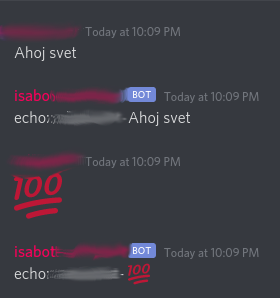
\includegraphics[width=10cm]{isabot.png}
    \label{fig:isabot}
\end{figure}

\newpage
\section{Bibliografia}
\bibliographystyle{czechiso}
\bibliography{manual}
\nocite{discord}
\nocite{stackoverflow}
\nocite{wiki_ssl}
\nocite{wiki_https}

\end{document}
